\section{Hadoop Open Plataform-as-a-Service (Hops)}

Hops is a new distribution of Apache Hadoop 2.x that has a new metadata management architecture based on a shared-nothing, in-memory distributed database, see Figure \ref{fig:hop-fs_architecture}, . 


Unlike HDFS (see figure \ref{fig:hdfs_architecture}), HopsFS has multiple NameNodes that manage the namespace metadata. All HopsFS' clients and DataNodes are aware of all NameNodes in the system. Whenever a NameNode fails the failed operations are automatically retried by clients and the DataNodes by forwarding the failed requests to a different live NameNode. In the remainder of this section we will present different architectural components of HopsFS, starting from the metadata storage layer, followed by the NameNodes, the DataNodes and the clients. 

\begin{figure}[h]
 \centering
 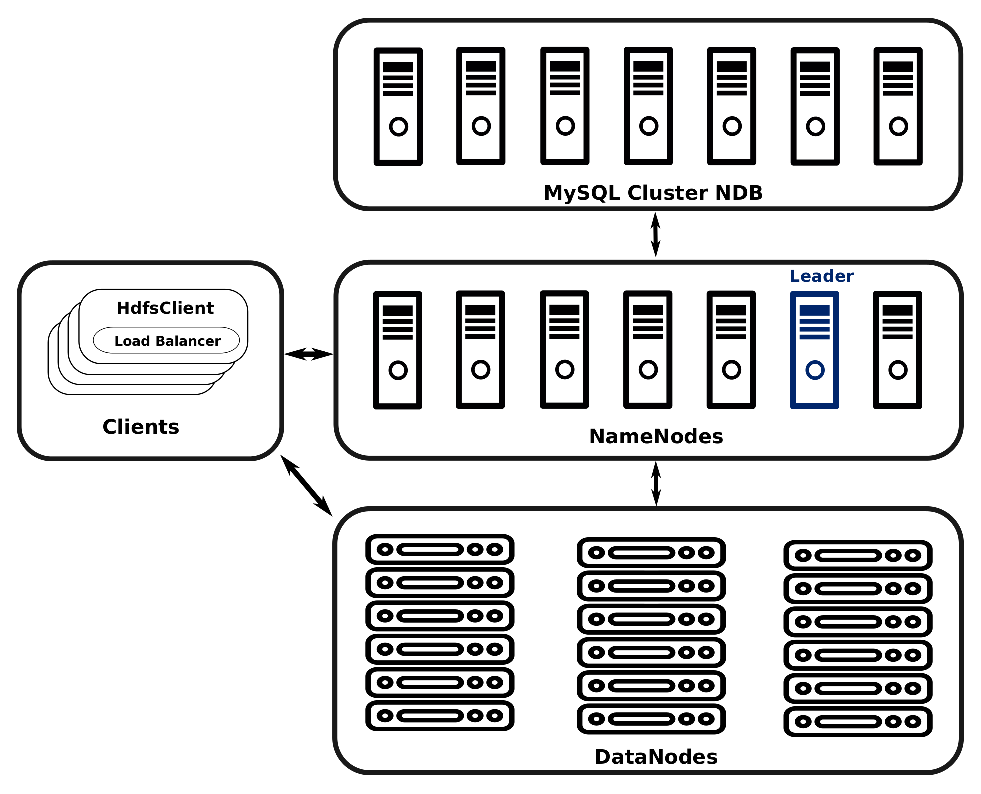
\includegraphics[width=0.9\textwidth]{./imgs/hops-fs-arch.eps}
 % hops-fs-arch.eps: 0x0 pixel, 300dpi, 0.00x0.00 cm, bb=0 -1 455 364
\end{figure}



% Jim - 1-3 pages
We have moved metadata from the heap of a Java Virtual Machine to an in-memory, no-shared-state, distributed database, called MySQL Cluster~\cite{ronstrom2005recovery}. 

We ensure the consistency of the filesystem metadata by implementing serialized transactions on well-ordered operations on metadata~\cite{hops_consistency}.

We do not need Zookeeper, as we have developed a leader-election service based on the database~\cite{hopselection}.


\begin{figure}[h]
 \centering
 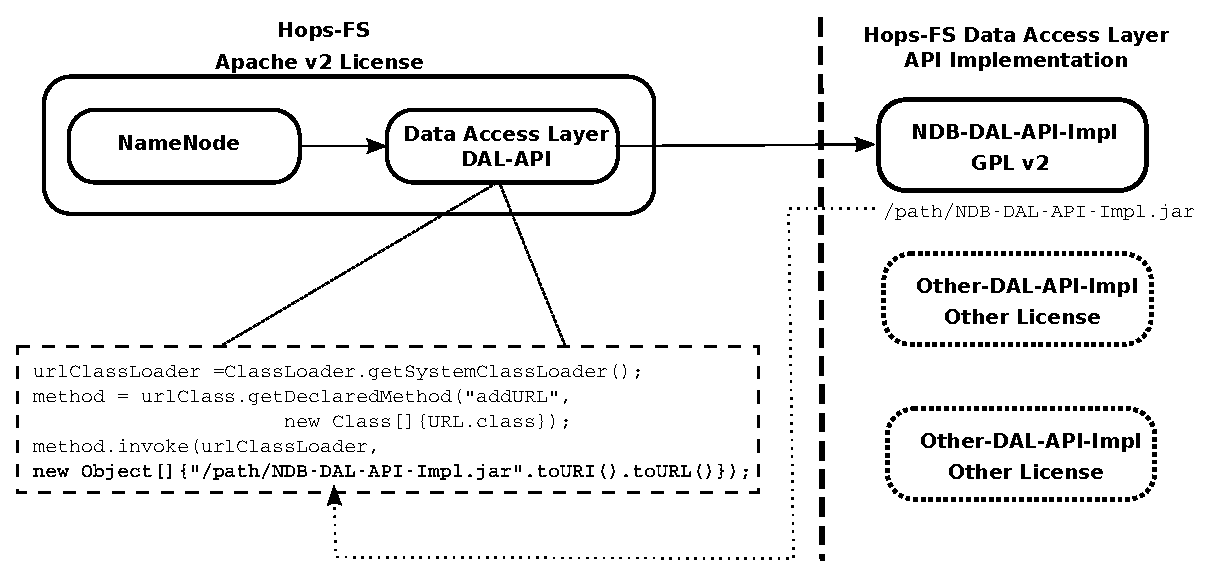
\includegraphics[width=0.9\textwidth]{./imgs/license-work-around.eps}
 \label{fig:license-work-around}
 \caption{Combining Apache v2 and GPL v2 Open Source Licenses}
 % license-work-around.eps: 0x0 pixel, 300dpi, 0.00x0.00 cm, bb=0 -1 566 261
\end{figure}


HopsFS reduces the storage cost of replication by supporting Reed-Solomon erasure coding to reduce the disk space consumption by 44\% compared to three-way replication of files used in Apache HDFS.


\begin{figure}[h]
 \centering
 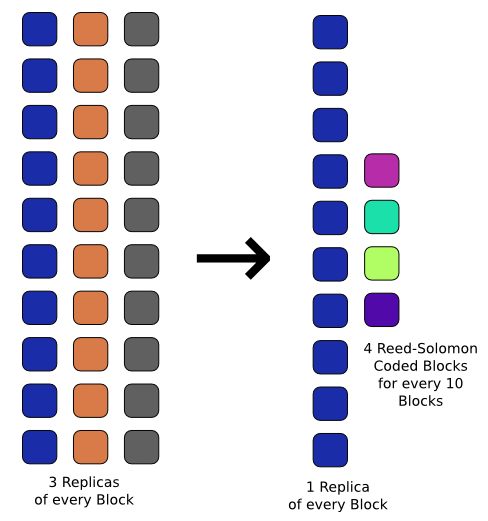
\includegraphics[width=0.5\textwidth]{./imgs/erasure-coding.png}
 % erasure-coding.png: 0x0 pixel, 300dpi, 0.00x0.00 cm, bb=
 \label{fig:erasure-coding}
 \caption{Storage savings through the application of erasure coding.}
\end{figure}
